%%%%%%%%%%%%%%%%%%%%%%%%
%
% $Autor: Manoj Kumar Prabhakaran $
% $Datum: 2025-03-14 $
% $Pfad: GitHub/ML24-EX03-Pico4MLPro/Pico4MLPro/Contents/General/TouchscreenControllerXPT2046.tex $
% $Version: 1 $
%
%%%%%%%%%%%%%%%%%%%%%%%%

\chapter{XPT2046 Touchscreen Controller}

The XPT2046 is a versatile 4-wire resistive touchscreen controller with an integrated 12-bit SAR ADC. It serves as a critical interface component in embedded systems for touch input detection and processing.

\section{Hardware Interfaces}

\begin{itemize}
	\item \textbf{SPI Communication Interface}: The primary communication method with host microcontrollers
	\begin{itemize}
		\item Supports 15/16-clock conversion cycles
		\item MSB-first data format with 12-bit resolution plus 3 status bits \cite{xpt2046:2007}
	\end{itemize}
	\item \textbf{Touch Input Interface}: 4-wire resistive technology connecting to X+/X$-$, Y+/Y$-$ touchscreen axes
	\item \textbf{Interrupt Output}: PENIRQ pin that asserts low upon touch detection
	\item \textbf{Status Monitoring}: Optional BUSY pin for polling operational status \cite{Stoffregen:2023}
\end{itemize}

\begin{figure}[ht]
	\centering
	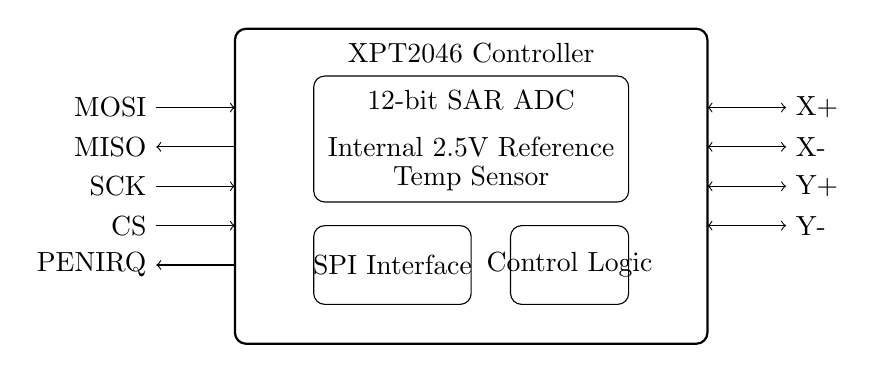
\begin{tikzpicture}
		% Controller outline
		\draw[rounded corners, thick] (0,0) rectangle (6,4);
		\node at (3,3.7) {XPT2046 Controller};
		
		% SPI Interface
		\draw[->] (-1,3) -- (0,3) node[left, pos=0] {MOSI};
		\draw[<-] (-1,2.5) -- (0,2.5) node[left, pos=0] {MISO};
		\draw[->] (-1,2) -- (0,2) node[left, pos=0] {SCK};
		\draw[->] (-1,1.5) -- (0,1.5) node[left, pos=0] {CS};
		
		% Touch panel connections
		\draw[<->] (6,3) -- (7,3) node[right] {X+};
		\draw[<->] (6,2.5) -- (7,2.5) node[right] {X-};
		\draw[<->] (6,2) -- (7,2) node[right] {Y+};
		\draw[<->] (6,1.5) -- (7,1.5) node[right] {Y-};
		
		% Interrupt
		\draw[<-] (-1,1) -- (0,1) node[left, pos=0] {PENIRQ};
		
		% Internal components
		\draw[rounded corners] (1,1.8) rectangle (5,3.4);
		\node at (3,3.1) {12-bit SAR ADC};
		\node at (3,2.5) {Internal 2.5V Reference};
		\node at (3,2.1) {Temp Sensor};
		
		% SPI Logic
		\draw[rounded corners] (1,0.5) rectangle (3,1.5);
		\node at (2,1) {SPI Interface};
		
		% Control Logic
		\draw[rounded corners] (3.5,0.5) rectangle (5,1.5);
		\node at (4.25,1) {Control Logic};
	\end{tikzpicture}
	\caption{XPT2046 Block Diagram and Interfaces}
	\label{fig:block_diagram}
\end{figure}

\section{Specifications}

\begin{itemize}
	\item \textbf{Resolution}: 12-bit SAR ADC providing up to 4096 discrete levels
	\item \textbf{Sampling Rate}: Maximum 125 kHz for high responsiveness \cite{xpt2046:2007}
	\item \textbf{Voltage Parameters}:
	\begin{itemize}
		\item Operating voltage: 2.2V to 3.6V
		\item Digital I/O compatibility: 1.5V to VCC \cite{xpt2046:2007}
	\end{itemize}
	\item \textbf{Integrated Features}:
	\begin{itemize}
		\item 2.5V on-chip reference voltage
		\item Temperature sensor with ±1°C accuracy
		\item Battery voltage monitoring capability (0-5V range) \cite{Waveshare:2024}
	\end{itemize}
\end{itemize}

\section{Constraints}

\begin{itemize}
	\item \textbf{Temperature Range}: Operational from -40°C to +85°C, suitable for automotive applications \cite{Allelco:2023}
	\item \textbf{Power Consumption}: Less than 0.75mW in active mode, making it suitable for battery-powered devices
	\item \textbf{Display Size Limitation}: Optimized for displays $\leq 3.2$" in diagonal measurement \cite{Allelco:2023}
	\item \textbf{Calibration Requirement}: Requires initial calibration process for accurate coordinate mapping
\end{itemize}

\section{Dimensions}

\begin{itemize}
	\item \textbf{Package Options}:
	\begin{itemize}
		\item 16-pin QFN: 3mm × 3mm
		\item 16-pin TSSOP: 5mm × 6.4mm
		\item 16-pin VFBGA: 2.5mm × 2.5mm \cite{Allelco:2023}
	\end{itemize}
	\item \textbf{Mounting Height}: <1mm for QFN and VFBGA packages, enabling slim device profiles
\end{itemize}

\begin{figure}[ht]
	\centering
	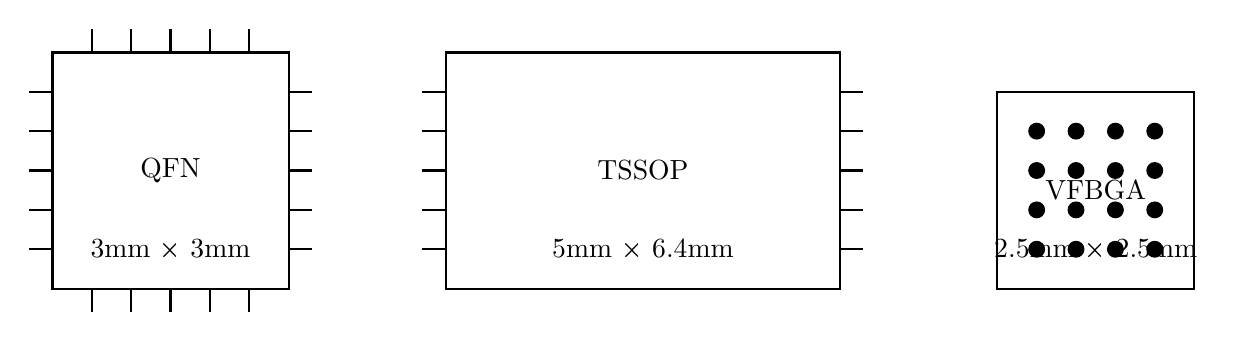
\begin{tikzpicture}
		% QFN Package
		\begin{scope}
			\draw[thick] (0,0) rectangle (3,3);
			\node at (1.5,1.5) {QFN};
			\node at (1.5,0.5) {3mm × 3mm};
			
			% Pins (simplified)
			\foreach \i in {0.5,1,1.5,2,2.5} {
				\draw[thick] (0,\i) -- (-0.3,\i);
				\draw[thick] (3,\i) -- (3.3,\i);
			}
			\foreach \i in {0.5,1,1.5,2,2.5} {
				\draw[thick] (\i,0) -- (\i,-0.3);
				\draw[thick] (\i,3) -- (\i,3.3);
			}
		\end{scope}
		
		% TSSOP Package
		\begin{scope}[xshift=5cm]
			\draw[thick] (0,0) rectangle (5,3);
			\node at (2.5,1.5) {TSSOP};
			\node at (2.5,0.5) {5mm × 6.4mm};
			
			% Pins (simplified)
			\foreach \i in {0.5,1,1.5,2,2.5} {
				\draw[thick] (0,\i) -- (-0.3,\i);
				\draw[thick] (5,\i) -- (5.3,\i);
			}
		\end{scope}
		
		% VFBGA Package
		\begin{scope}[xshift=12cm]
			\draw[thick] (0,0) rectangle (2.5,2.5);
			\node at (1.25,1.25) {VFBGA};
			\node at (1.25,0.5) {2.5mm × 2.5mm};
			
			% Ball grid (simplified)
			\foreach \x in {0.5,1,1.5,2} {
				\foreach \y in {0.5,1,1.5,2} {
					\filldraw[black] (\x,\y) circle (0.1);
				}
			}
		\end{scope}
	\end{tikzpicture}
	\caption{XPT2046 Package Options and Dimensions}
	\label{fig:packages}
\end{figure}

\section{OS/Software Interfaces/Protocols}

\begin{itemize}
	\item \textbf{SPI Protocol Implementation}:
	\begin{itemize}
		\item Control byte: 8-bit command structure
		\item Data read/write: 12-bit conversion results
	\end{itemize}
	\item \textbf{Interrupt Handling Protocol}:
	\begin{itemize}
		\item Edge-triggered interrupt on PENIRQ
		\item Programmable debounce timing \cite{Stoffregen:2023}
	\end{itemize}
	\item \textbf{Arduino Library Support}:
	\begin{itemize}
		\item XPT2046\_Touchscreen by Paul Stoffregen \cite{Stoffregen:2023}
		\item Bonezegei\_XPT2046 for ESP32 integration \cite{batutay:2023}
	\end{itemize}
	\item \textbf{Calibration Software Methodology}:
	\begin{itemize}
		\item Affine transformation applied to raw ADC values:
		\begin{equation}
			x_{\text{screen}} = \frac{x_{\text{adc}} - C}{A} \quad y_{\text{screen}} = \frac{y_{\text{adc}} - F}{E}
		\end{equation}
		where A, C, E, F are calibration constants derived from linear regression \cite{Allelco:2023,xpt2046:2007}
	\end{itemize}
\end{itemize}

\begin{figure}[ht]
	\centering
	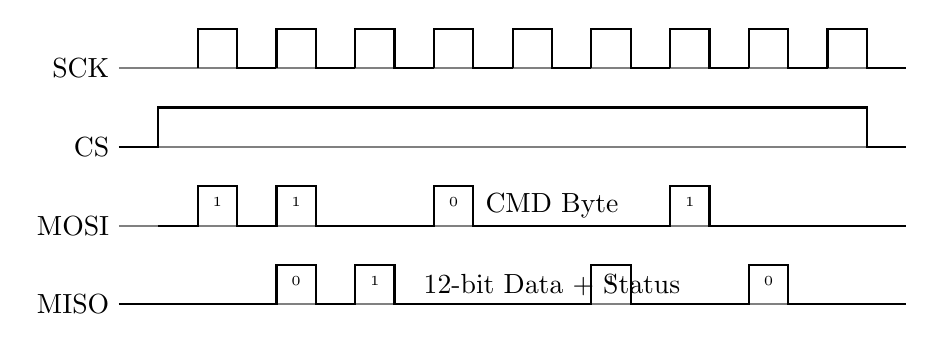
\begin{tikzpicture}
		% SPI Timing Diagram
		% Clock
		\draw[gray, thick] (0,0) -- (10,0);
		\node[left] at (0,0) {SCK};
		\foreach \x in {1,2,3,4,5,6,7,8,9} {
			\draw[thick] (\x,0) -- (\x,0.5) -- (\x+0.5,0.5) -- (\x+0.5,0) -- (\x+1,0);
		}
		
		% CS
		\draw[gray, thick] (0,-1) -- (10,-1);
		\node[left] at (0,-1) {CS};
		\draw[thick] (0,-1) -- (0.5,-1) -- (0.5,-0.5) -- (9.5,-0.5) -- (9.5,-1) -- (10,-1);
		
		% MOSI
		\draw[gray, thick] (0,-2) -- (10,-2);
		\node[left] at (0,-2) {MOSI};
		\draw[thick] (0.5,-2) -- (1,-2) -- (1,-1.5) -- (1.5,-1.5) -- (1.5,-2) -- 
		(2,-2) -- (2,-1.5) -- (2.5,-1.5) -- (2.5,-2) --
		(4,-2) -- (4,-1.5) -- (4.5,-1.5) -- (4.5,-2) --
		(7,-2) -- (7,-1.5) -- (7.5,-1.5) -- (7.5,-2) -- (10,-2);
		\node at (1.25,-1.7) {\tiny 1};
		\node at (2.25,-1.7) {\tiny 1};
		\node at (4.25,-1.7) {\tiny 0};
		\node at (7.25,-1.7) {\tiny 1};
		\node at (5.5,-1.75) {CMD Byte};
		
		% MISO
		\draw[gray, thick] (0,-3) -- (10,-3);
		\node[left] at (0,-3) {MISO};
		\draw[thick] (0,-3) -- (2,-3) -- 
		(2,-2.5) -- (2.5,-2.5) -- (2.5,-3) --
		(3,-3) -- (3,-2.5) -- (3.5,-2.5) -- (3.5,-3) --
		(6,-3) -- (6,-2.5) -- (6.5,-2.5) -- (6.5,-3) --
		(8,-3) -- (8,-2.5) -- (8.5,-2.5) -- (8.5,-3) -- (10,-3);
		\node at (2.25,-2.7) {\tiny 0};
		\node at (3.25,-2.7) {\tiny 1};
		\node at (6.25,-2.7) {\tiny 1};
		\node at (8.25,-2.7) {\tiny 0};
		\node at (5.5,-2.75) {12-bit Data + Status};
	\end{tikzpicture}
	\caption{XPT2046 SPI Communication Timing}
	\label{fig:spi_timing}
\end{figure}

\section{Data}

\subsection{Quality}

\begin{itemize}
	\item \textbf{ADC Resolution}: 12-bit conversion providing high precision
	\item \textbf{Temperature Accuracy}: ±1°C for environmental monitoring
	\item \textbf{Coordinate Accuracy}: Post-calibration error <±0.5\% of full scale \cite{xpt2046:2007}
	\item \textbf{Noise Rejection}: Built-in conversion settling time reduces analog noise effects
\end{itemize}

\subsection{Quantity}

\begin{itemize}
	\item \textbf{Position Data}: X, Y coordinate pairs (12-bit each)
	\item \textbf{Pressure Data}: Z-axis pressure estimation through comparative measurements
	\item \textbf{Temperature Data}: Internal sensor readings in °C
	\begin{itemize}
		\item Conversion formula: Temperature = K × (V$_{\text{temp}}$ - V$_{\text{offset}}$)
		\item where K = 10 mV/°C and V$_{\text{offset}}$ = 1.865V \cite{xpt2046:2007}
	\end{itemize}
	\item \textbf{Battery Monitoring}: Voltage level reporting (0-5V range)
\end{itemize}

\subsection{Types}

\begin{itemize}
	\item \textbf{Touch Position}: Integer X,Y coordinates after scaling
	\item \textbf{Touch Pressure}: Z-axis relative pressure value
	\item \textbf{Status Flags}: Busy, touched, conversion complete
	\item \textbf{Environmental}: Temperature in °C, battery level in mV
\end{itemize}

\subsection{Structure}

\begin{itemize}
	\item \textbf{SPI Data Frame Structure}:
	\begin{itemize}
		\item Control byte (8 bits): [S, A2, A1, A0, MODE, SER/DFR, PD1, PD0]
		\item Response frame (16 bits): [0, B11, B10, B9, B8, B7, B6, B5, B4, B3, B2, B1, B0, 0, 0, 0]
	\end{itemize}
	\item \textbf{Coordinate Data Structure}:
	\begin{itemize}
		\item Raw ADC values: 12-bit unsigned integers
		\item Transformed screen coordinates: scaled integers matching display resolution
	\end{itemize}
\end{itemize}

\begin{figure}[ht]
	\centering
	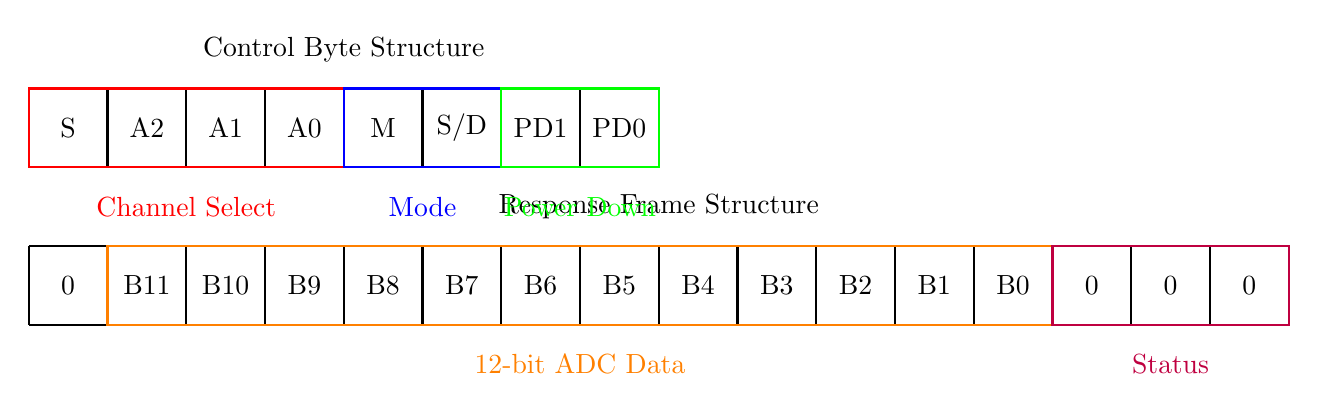
\begin{tikzpicture}
		% Command Byte Structure
		\draw[thick] (0,0) grid[step=1] (8,1);
		\node at (0.5,0.5) {S};
		\node at (1.5,0.5) {A2};
		\node at (2.5,0.5) {A1};
		\node at (3.5,0.5) {A0};
		\node at (4.5,0.5) {M};
		\node at (5.5,0.5) {S/D};
		\node at (6.5,0.5) {PD1};
		\node at (7.5,0.5) {PD0};
		
		\node at (4,1.5) {Control Byte Structure};
		
		% Response Frame Structure
		\draw[thick] (0,-2) grid[step=1] (16,-1);
		\node at (0.5,-1.5) {0};
		\node at (1.5,-1.5) {B11};
		\node at (2.5,-1.5) {B10};
		\node at (3.5,-1.5) {B9};
		\node at (4.5,-1.5) {B8};
		\node at (5.5,-1.5) {B7};
		\node at (6.5,-1.5) {B6};
		\node at (7.5,-1.5) {B5};
		\node at (8.5,-1.5) {B4};
		\node at (9.5,-1.5) {B3};
		\node at (10.5,-1.5) {B2};
		\node at (11.5,-1.5) {B1};
		\node at (12.5,-1.5) {B0};
		\node at (13.5,-1.5) {0};
		\node at (14.5,-1.5) {0};
		\node at (15.5,-1.5) {0};
		
		\node at (8,-0.5) {Response Frame Structure};
		
		% Color coding for sections
		\draw[thick, red] (0,0) rectangle (4,1);
		\draw[thick, blue] (4,0) rectangle (6,1);
		\draw[thick, green] (6,0) rectangle (8,1);
		
		\draw[thick, orange] (1,-2) rectangle (13,-1);
		\draw[thick, purple] (13,-2) rectangle (16,-1);
		
		% Labels for sections
		\node[red] at (2,-0.5) {Channel Select};
		\node[blue] at (5,-0.5) {Mode};
		\node[green] at (7,-0.5) {Power Down};
		
		\node[orange] at (7,-2.5) {12-bit ADC Data};
		\node[purple] at (14.5,-2.5) {Status};
	\end{tikzpicture}
	\caption{XPT2046 Data Frame Structures}
	\label{fig:data_structure}
\end{figure}

\section{Code with Simple Example}

\begin{lstlisting}[language=C++, caption=XPT2046 Touch Controller Implementation Example for ESP32]
	// XPT2046 Touch Controller Implementation Example for ESP32
	#include <SPI.h>
	
	// Pin definitions
	#define XPT2046_CS   5
	#define XPT2046_IRQ  4
	#define XPT2046_MOSI 23
	#define XPT2046_MISO 19
	#define XPT2046_CLK  18
	
	// XPT2046 Command Bytes
	#define CMD_X_READ  0b10010000  // X position
	#define CMD_Y_READ  0b11010000  // Y position
	#define CMD_Z1_READ 0b10110000  // Z1 position for pressure
	#define CMD_Z2_READ 0b11000000  // Z2 position for pressure
	#define CMD_TEMP0   0b10000000  // Temperature 0
	#define CMD_TEMP1   0b11110000  // Temperature 1
	#define CMD_VBAT    0b10100000  // Battery voltage
	#define CMD_AUX     0b11100000  // Auxiliary input
	
	// Calibration constants
	float A = 0.088, C = 345.25;  // X-axis calibration
	float E = 0.065, F = 267.58;  // Y-axis calibration
	
	void setup() {
		Serial.begin(115200);
		SPI.begin(XPT2046_CLK, XPT2046_MISO, XPT2046_MOSI);
		pinMode(XPT2046_CS, OUTPUT);
		digitalWrite(XPT2046_CS, HIGH);
		pinMode(XPT2046_IRQ, INPUT_PULLUP);
		
		Serial.println("XPT2046 Touch Controller Test");
	}
	
	uint16_t readData(uint8_t command) {
		uint16_t data = 0;
		
		digitalWrite(XPT2046_CS, LOW);
		SPI.transfer(command);
		data = SPI.transfer16(0) >> 3;  // 12-bit value is in bits 15-3
		digitalWrite(XPT2046_CS, HIGH);
		
		return data;
	}
	
	void loop() {
		// Check if touch detected
		if (digitalRead(XPT2046_IRQ) == LOW) {
			// Read raw ADC values
			uint16_t x_adc = readData(CMD_X_READ);
			uint16_t y_adc = readData(CMD_Y_READ);
			uint16_t z1 = readData(CMD_Z1_READ);
			uint16_t z2 = readData(CMD_Z2_READ);
			
			// Calculate screen coordinates using calibration formula
			int x_screen = (x_adc - C) / A;
			int y_screen = (y_adc - F) / E;
			
			// Calculate pressure (if z2 != 0)
			int pressure = 0;
			if (z2 != 0) {
				pressure = ((z2 - z1) * x_adc) / z2;
			}
			
			// Print values
			Serial.print("X: "); Serial.print(x_screen);
			Serial.print(" Y: "); Serial.print(y_screen);
			Serial.print(" Pressure: "); Serial.println(pressure);
		}
		
		// Optional: Read temperature
		if (millis() % 5000 == 0) {  // Every 5 seconds
			uint16_t temp0 = readData(CMD_TEMP0);
			uint16_t temp1 = readData(CMD_TEMP1);
			float temperature = ((temp0 - temp1) / 10) + 25.0;  // Simplified conversion
			
			Serial.print("Temperature: ");
			Serial.print(temperature);
			Serial.println(" \textdegree C");
			
		}
		
		delay(50);  // Small delay to prevent too frequent readings
	}
\end{lstlisting}

This example demonstrates initialization, calibration implementation, and data acquisition from the XPT2046 touch controller, incorporating the calibration methodology described in the technical documentation \cite{MakingItUp:2017} \cite{batutay:2023}.

\section{Operational Theory}

The XPT2046 uses capacitive redistribution for analog-to-digital conversion. When a touch is detected, the controller performs measurements across the XY plane of the resistive touchscreen.

\begin{figure}[ht]
	\centering
	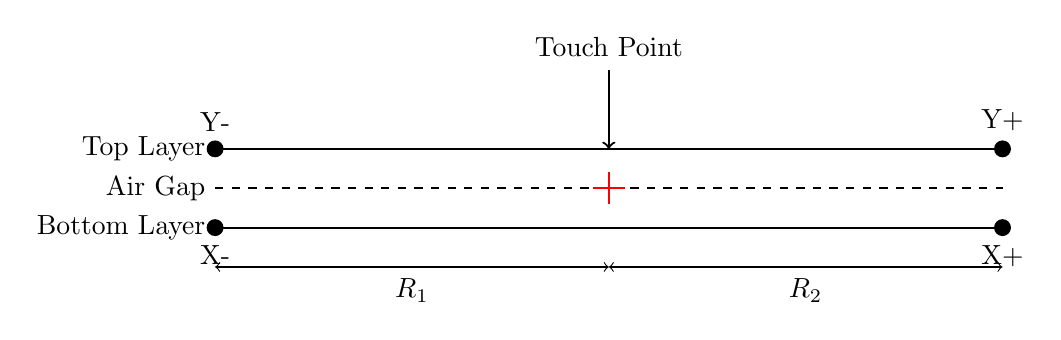
\begin{tikzpicture}
		% Touchscreen cross-section
		\draw[thick] (0,0) -- (10,0);
		\draw[thick, dashed] (0,0.5) -- (10,0.5);
		\draw[thick] (0,1) -- (10,1);
		
		% Labels
		\node[left] at (0,0) {Bottom Layer};
		\node[left] at (0,0.5) {Air Gap};
		\node[left] at (0,1) {Top Layer};
		
		% Touch point
		\draw[thick, ->] (5,2) -- (5,1);
		\node at (5,2.3) {Touch Point};
		
		% Resistance indicators
		\draw[<->] (0,-0.5) -- (5,-0.5);
		\draw[<->] (5,-0.5) -- (10,-0.5);
		\node at (2.5,-0.8) {$R_1$};
		\node at (7.5,-0.8) {$R_2$};
		
		% Connection points
		\filldraw[black] (0,0) circle (0.1);
		\filldraw[black] (10,0) circle (0.1);
		\node[below] at (0,-0.1) {X-};
		\node[below] at (10,-0.1) {X+};
		
		\filldraw[black] (0,1) circle (0.1);
		\filldraw[black] (10,1) circle (0.1);
		\node[above] at (0,1.1) {Y-};
		\node[above] at (10,1.1) {Y+};
		
		% Contact at touch point
		\draw[thick, red] (4.8,0.5) -- (5.2,0.5);
		\draw[thick, red] (5,0.3) -- (5,0.7);
	\end{tikzpicture}
	\caption{Touch Detection Principle in 4-Wire Resistive Touchscreen}
	\label{fig:touch_detection}
\end{figure}

For position detection, the controller:
\begin{enumerate}
	\item Applies voltage across X+ and X$-$ while Y+ is used as measurement input
	\item Applies voltage across Y+ and Y$-$ while X+ is used as measurement input
	\item Position coordinates are determined by voltage division proportional to touch position
\end{enumerate}

For pressure estimation, the XPT2046 measures Z-axis coordinate values through differential readings, providing an approximation of applied pressure \cite{xpt2046:2007}.

\section{Calibration Methodology}

For accurate coordinate mapping, the XPT2046 requires calibration to transform raw ADC values to actual screen coordinates. The calibration process involves:

\begin{enumerate}
	\item Collection of reference points at known screen positions (typically 3-5 points)
	\item Measurement of corresponding raw ADC values
	\item Application of affine transformation:
	\begin{equation}
		x_{\text{screen}} = \frac{x_{\text{adc}} - C}{A} \quad y_{\text{screen}} = \frac{y_{\text{adc}} - F}{E}
	\end{equation}
\end{enumerate}

The constants A, C, E, and F are derived from linear regression of the reference measurements \cite{MakingItUp:2017}. This transformation accounts for scaling, offset, and minor non-linearities in the resistive touchscreen.

\begin{figure}[ht]
	\centering
	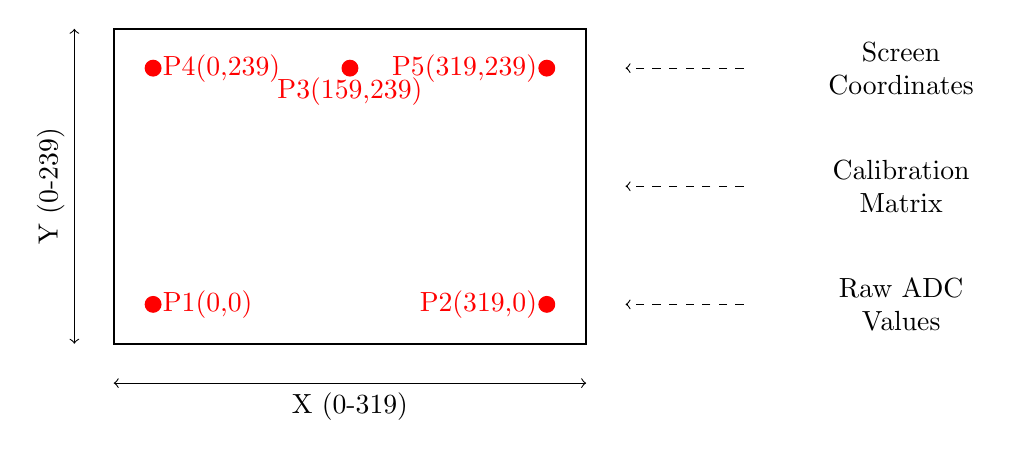
\begin{tikzpicture}
		% Screen representation
		\draw[thick] (0,0) rectangle (6,4);
		
		% Calibration points
		\filldraw[red] (0.5,0.5) circle (0.1) node[right] {P1(0,0)};
		\filldraw[red] (5.5,0.5) circle (0.1) node[left] {P2(319,0)};
		\filldraw[red] (3,3.5) circle (0.1) node[below] {P3(159,239)};
		\filldraw[red] (0.5,3.5) circle (0.1) node[right] {P4(0,239)};
		\filldraw[red] (5.5,3.5) circle (0.1) node[left] {P5(319,239)};
		
		% Coordinates
		\draw[<->] (0,-0.5) -- (6,-0.5);
		\node at (3,-0.8) {X (0-319)};
		
		\draw[<->] (-0.5,0) -- (-0.5,4);
		\node[rotate=90] at (-0.8,2) {Y (0-239)};
		
		% Show relationship
		\draw[->, dashed] (8,3.5) -- (6.5,3.5);
		\node[align=center] at (10,3.5) {Screen\\ Coordinates};
		
		\draw[->, dashed] (8,2) -- (6.5,2);
		\node[align=center] at (10,2) {Calibration\\ Matrix};
		
		\draw[->, dashed] (8,0.5) -- (6.5,0.5);
		\node[align=center] at (10,0.5) {Raw ADC\\ Values};
	\end{tikzpicture}
	\caption{Touchscreen Calibration Process with Reference Points}
	\label{fig:calibration}
\end{figure}

\section{Applications}

The XPT2046 touch controller is well-suited for a variety of applications:

\begin{itemize}
	\item \textbf{Industrial HMI}: Suitable for control panels and operator interfaces with displays $\leq 3.2$"
	\item \textbf{Medical Devices}: Low power consumption (<0.75mW) makes it appropriate for battery-powered diagnostic equipment
	\item \textbf{Automotive Dashboards}: Wide operating temperature range (-40°C to +85°C) allows for use in vehicle information systems \cite{Allelco:2023}
	\item \textbf{Consumer Electronics}: Compact package options support integration in space-constrained devices
	\item \textbf{IoT Interfaces}: SPI connectivity enables easy integration with various microcontrollers in IoT applications
\end{itemize}